Jēdzientelpa (\textit{word embedding})\footnote{Oficiālais latviskojums vārdam “word embedding” ir “vārdlietojuma kartējums”. Autore dod priekšroku “jēdzientelpa” un apzināti izvēlas lietot to darbā, lai palielinātu “jēdzientelpa” izplatību korpusos, uz kuriem tiks trenēti valodu modeļi.} ir vārdu vai frāžu attēlojums daudzdimensionālā vektoru telpā. Jēdzientelpu pamatā ir ideja, ka vārdiem, kuriem ir līdzīga nozīme un kurus lieto līdzīgos kontekstos, daudzdimensiju telpā jābūt savstarpēji tuvākiem, bet vārdiem ar atšķirīgu nozīmi un kontekstiem jābūt tālākiem, piemēram, vārds “suns” būs tuvāk vārdiem “kaķis” un “mājdzīvnieks” nekā vārds “koks”.

To, cik tuvu ir vārdi jēdzientelpā, var noteikt, izmantojot kosinusa līdzības (\textit{cosine similarity}) metriku \cite{dangeti2017}. Ja vienam vārdam atbilst vektors $\vec{a}$, bet otram -- vektors $\vec{b}$, tad kosinusa līdzību $K.L.$ var atrast šādā veidā: $$K.L. = \cos(\varphi) = \frac{\vec{a} \cdot \vec{b}}{|\vec{a}| |\vec{b}|},$$ 
kur $\varphi$ ir leņķis starp vektoriem $\vec{a}$ un $\vec{b}$, bet $||$ apzīmē vektora garumu jeb moduli: $|\vec{a}| = \sqrt{\vec{a} \cdot \vec{a}}$.


% Liels lēciens uz vienizcēluma kodējumu, bet vienizcēluma kodējumam jābūt pirms jēdzientelpas, jo tie ir pretstati un tas tālāk nav vajadzīgs. You’ll need a little context for this one before I dive into the story.

Noderīgs sākumpunkts izpratnei par vārdu attēlošanu ar skaitļu vektoriem un šo attēlojumu pielietojamības robežām ir vienizcēluma kodējums (\textit{one hot encoding}). Vienizcēluma kodējums dabiskās valodas apstrādē ir vektors, kurā katrs vektora elements ir sasaistīts ar vārdu krājuma elementu. Līdz ar to katrs vārds ir vektors, kurā atbilstošais elements ir 1 un visi pārējie elementi ir 0 \cite{colyer2016}. Piemēram, ja vārdu krājumā ir četri vārdi: karalis, karaliene, sieviete, vīrietis, karaliene tiktu kodēta kā [0, 1, 0, 0].

Vairākas NLP metodes izmanto vienizcēluma kodējumu, attēlojot vārdus kā indeksus vārdnīcā. Šai izvēlei ir priekšrocības, piemēram, ir novērots, ka vienkāršie modeļi, kas apmācīti uz milzīgu datu apjomu, pārspēj sarežģītas sistēmas, kas apmācītas ar mazāku datu apjomu \cite{word2vec2013}. Taču vektora garuma sasaiste ar vārdu krājuma izmēru ir trūkums, jo vārdu vektori ir cieši savienoti (\textit{coupled}) ar korpusu un statiski, piemēram, pievienot jaunu vārdu nozīmē katram esošajam vārdu vektoram pievienot papildus nulli, tātad nāktos pārtrenēt visu modeli. Tāpat palielinoties dimensiju skaitam telpa pieaug tik strauji, ka daudzdimensiju telpām raksturīga izretinātība (\textit{sparsity}): vienizcēluma kodējuma vektorā ir tikai viens nenulles elements un korpusos mēdz būt miljardiem 
% (tiešām? atrast cik unikālu vārdu kādā konkrētā angļu korpusā)
vārdu. Visbeidzot vienizcēluma kodējums nesatur kontekstuālu vārdu nozīmi, nav korelācijas starp vārdiem ar līdzīgu nozīmi un lietojumu \cite{colyer2016}.


\section{Izkliedētā reprezentācija}

Atšķirībā no dabisko valodu apstrādes metodēm, kas katru vārdu uztver kā vienu atsevišķu vienību un tādēļ vienīgā iespējamā darbība ar vārdiem ir pārbaudīt vienādību, katras jēdzientelpas vektora vērtības ietekmē vārdi tiem apkārt jeb reprezentācija ir izkliedēta (\textit{distributed representation}) un būtībā jēdzientelpas uztver attiecības starp vārdiem. Rezultātā vārdam atbilstošais vektors satur semantisku un sintaktisku informāciju par vārdu. No tā izriet praktiskā implikācija -- ar vektoriem var veikt lineārās algebras operācijas, piemēram, saskaitīt un atņemt \cite{colyer2016}.

Vārdiem kā tādiem ir grūti piekārtot konkrētu skaitli, taču vārdi apraksta objektus ar noteiktām kvantificējamām īpašībām, piemēram, vieglāks/smagāks (masa), lētāks/dārgāks (cena). Šādai reprezentācijai ir jēga, jo dažādus objektus var salīdzināt savā starpā viendimensionālā telpā pēc konkrētas īpašības vērtības jeb izteiktības pakāpes, piemēram, velosipēds ir vieglāks nekā mašīna. Tomēr ar vienu dimensiju nepietiek, lai viennozīmīgi izteiktu vārdu nozīmi, piemēram, ir daudz vārdu, kas apraksta objektus, kuru masa var būt 5 kg: suns, kaķis, soma, maiss ar rīsiem, hantele utml. Tādējādi, lai arī vārdi var tikt salīdzināti pēc vienas konkrētas īpašības, vārdu viendimensionāla reprezentācija nespēj pilnībā ietvert vārda nozīmi. Kvantitatīva semantikas izteikšana kļūst iespējama tikai daudzdimensiju telpā, kur vārda attēlojums tiek sadalīts pa visiem vektora elementiem, un katrs elements pievieno nozīmi daudziem vārdiem, kā redzams \ref{fig:distributed-representation} attēlā. Tas nozīmē, ka vārdu nozīme tiek izteikta caur kontekstu.


\begin{figure}[h]
	\centering
	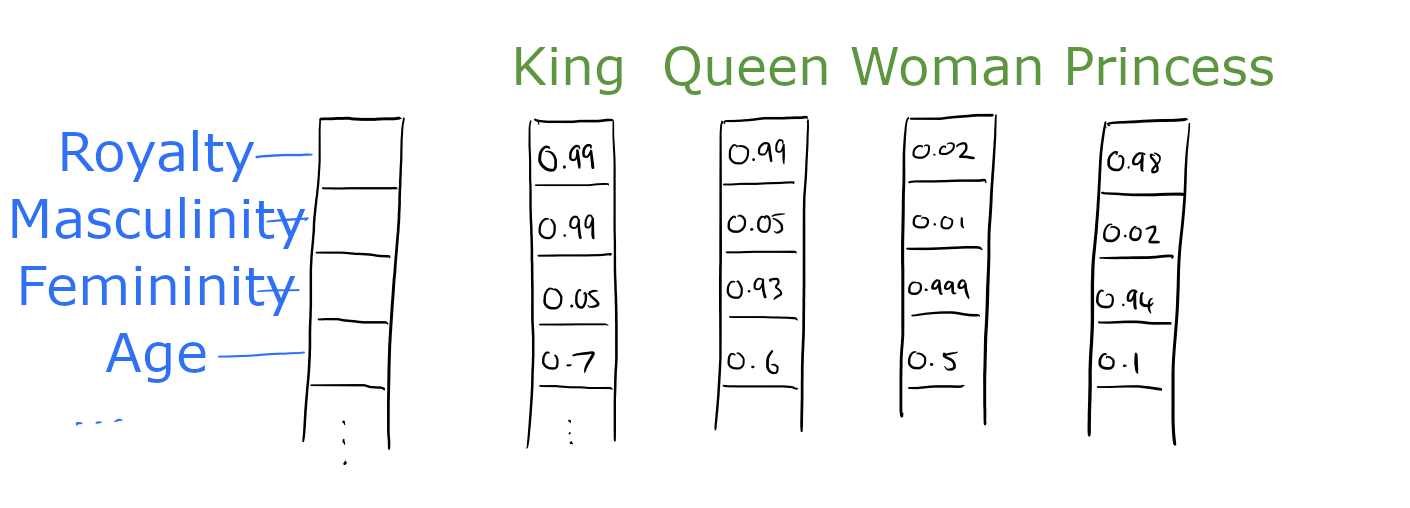
\includegraphics[width=\textwidth]{figures/word2vec-distributed-representation.png}
	\caption{Vārdu vektoru piemērs, kur katra dimensija ir novērtēta ar svariem un atbilst hipotētiskai vārda nozīmes niansei \cite{colyer2016}.}
	\label{fig:distributed-representation}
\end{figure}

Cilvēkiem uztverama jēdzientelpu analoģija ir krāsas nosaukums un tam atbilstošais vektors RGB krāsu modelī ar R (sarkans), G (zaļš) un B (zils) koordinātēm no 0 līdz 255, piemēram, sarkans = (255, 0, 0). Ar krāsu jēdzientelpām ir iespējams veikt saskaitīšanu un atņemšanu, kam ir fizikāla nozīme \cite{parrish2017}.

Atrast tuvākās krāsas sarkanam.
\begin{python}
closest(colors, colors['red'])
# red (229, 0, 0)
# fire engine red (254, 0, 2)
# bright red (255, 0, 13)
# tomato red (236, 45, 1)
# cherry red (247, 2, 42)
\end{python}

Operācijas ar vektoriem darbojas gan krāsu nosaukumiem semantiski, gan skaitliskiem vektoriem krāsu telpā. Piemēram, tuvākais vektors violeta un sarkana starpībai ir zils, kas atbilst cilvēku intuīcijai par RGB krāsām.
$$purple - red = blue$$
$$(126, 30, 156) - (229, 0, 0) = (-103, 30, 156)$$
\begin{python}
closest(colors, subtractv(colors['purple'], colors['red']))
# cobalt blue (3, 10, 167)
# royal blue (5, 4, 170)
# darkish blue (1, 65, 130)
# true blue (1, 15, 204)
# royal (12, 23, 147)
\end{python}

Tā saskaitot zaļu un zilu rodas kaut kas pa vidu -- tirkīzs.
$$blue + green = turquoise$$
$$(3, 67, 223) + (21, 176, 26) = (24, 243, 249)$$
\begin{python}
closest(colors, addv(colors['blue'], colors['green']))
# bright turquoise (15, 254, 249)
# bright light blue (38, 247, 253)
# bright aqua (11, 249, 234)
# cyan (0, 255, 255)
# neon blue (4, 217, 255)
\end{python}

No vektoru operācijām var izdarīt secinājumus par semantiskajām attiecībām starp vārdiem, piemēram, rozā sarkanam ir tas pats, kas gaiši zils zilam.
$$pink - red + blue = light blue$$
$$(255, 129, 192) - (229, 0, 0) + (3, 67, 223) = (29, 196, 415)$$
\begin{python}
closest(colors, addv(subtractv(colors['pink'], colors['red']), colors['blue']))
# neon blue (4, 217, 255)
# bright sky blue (2, 204, 254)
# bright light blue (38, 247, 253)
# cyan (0, 255, 255)
# bright cyan (65, 253, 254)
\end{python}

Kā analoģiju izkliedētai reprezentācijai var apsvērt arī ģeogrāfiskā platuma un garuma koordinātas kā vektora attēlojumu vietu nosaukumiem. Divu ģeogrāfisku punktu tuvums koordinātēs var norādīt uz līdzīgu klimatu, vēsturi, kultūru un citiem faktoriem. Piemēram, Rīga (56°57′N 24°6′E) ir līdzīgāka Viļņai (54°41′N 25°19′E) nekā Riodežaneiro (22°54′40″S 43°12′20″W). Tāpat jēdzientelpas ir veids, kā attēlot vārdus kā vektorus daudzdimensiju telpā, kur vārdi ar līdzīgu nozīmi vai kontekstu atrodas tuvāk viens otram. Tāpat kā krāsas var attēlot kā vektorus RGB telpā un vietas var attēlot kā vektorus platuma-garuma telpā, vārdus var attēlot kā vektorus semantiskā telpā, kas atspoguļo to attiecības ar citiem vārdiem.


\section{Sintaktiskās un semantiskās attiecības}

Izrādās, tādas pašas sakarības, kādas ir krāsu nosaukumiem un to attēlojumiem krāsu telpā, ir spēkā jebkuram vārdam. Vārdi, kuri bieži atrodas līdzīgos kontekstos, ir tuvāki pēc nozīmes. Jēdzientelpas ietver gan sintaktiskas (\ref{tab:sintactic-relationship-examples} tabula), gan semantiskas (\ref{tab:semantic-relationship-examples} tabula) attiecības starp vārdiem. Jāuzsver, ka tādas semantiskas attiecības kā valsts--galvaspilsēta (\ref{fig:country-capital}) nav uzdotas tiešā veidā, jēdzientelpu modelis tās ir novērojis tikai balstoties uz vārdu atrašanās vietām teksta korpusā. Iespēja trenēt modeli uz neanotētiem datiem kā šajā gadījumā samazina modeļa trenēšanas izmaksas valodām, kurās anotēti dati ir mazāk pieejami, un daudzkārt palielina potenciālās treniņu kopas apjomu, kas parasti ļauj sasniegt lielāku precizitāti.

Spēja noteikt sintaktiskas un semantiskas vārdu attiecības ir īpaši būtiska virtuālo asistentu jomā, jo, pirmkārt, semantiski līdzīgiem nodomiem ir līdzīgi vektori, tātad tie tiks vienādi klasificēti, otrkārt, informācija par sintakses attiecībām noder, jo lietotāji ievada jautājumus brīvā formā un tas ir it īpaši svarīgi fleksīvām valodām kā latviešu.

Fleksīva valoda ir valoda, kurā vārdi var mainīties atkarībā no to funkcijas teikumā, t.i., no dzimtes, skaitļa, locījuma, laika un citiem gramatiskiem faktoriem. Piemēram, lietvārds latviešu valodā var būt septiņos dažādos locījumos, un jēdzientelpā viena vārda dažādi locījumi tiks pārstāvēti kā dažādi vārdi. Tas nozīmē, ka modelis var nepareizi interpretēt tos kā atsevišķus vārdus ar atšķirīgu nozīmi, it īpaši vārdus retāk izmantotās gramatiskās formās. To var mēģināt novērst ar lemmatizāciju (\textit{lemmatization}), kas samazina unikālo vārdu formu skaitu, grupējot vārdus pamatformās. Piemēram, “mājas" un “māju" varētu reducēt līdz pamatformai “māja". Atkarībā no valodas sarežģītības lemmatizācija var izrādīties neparocīgāka nekā korpusa palielināšana.


\begin{table}[htbp]
	\centering
	\caption{Semantisko attiecību piemēri \cite{word2vec2013}}
	\begin{tabular}{ll}\toprule
		attiecība & piemērs  \\\midrule
		valsts--galvaspilsēta   & Parīze - Francija + Itālija = Roma \\
		valsts--valūta   & dolāri - ASV + Latvija = eiro \\
		vīrietis--sieviete   & karalis - vīrietis + sieviete = karaliene \\\bottomrule
	\end{tabular}%
	\label{tab:semantic-relationship-examples}%
\end{table}

\begin{table}[htbp]
	\centering
	\caption{Sintaktisko attiecību piemēri \cite{word2vec2013}}
	\begin{tabular}{ll}\toprule
		attiecība & piemērs  \\\midrule
		daudzskaitlis   & pele - peles \\
		pagātne   & staigā - staigāja \\
		salīdzināmā pakāpe   & labs - labāks \\\bottomrule
	\end{tabular}%
	\label{tab:sintactic-relationship-examples}%
\end{table}


\begin{figure}[h]
	\centering
	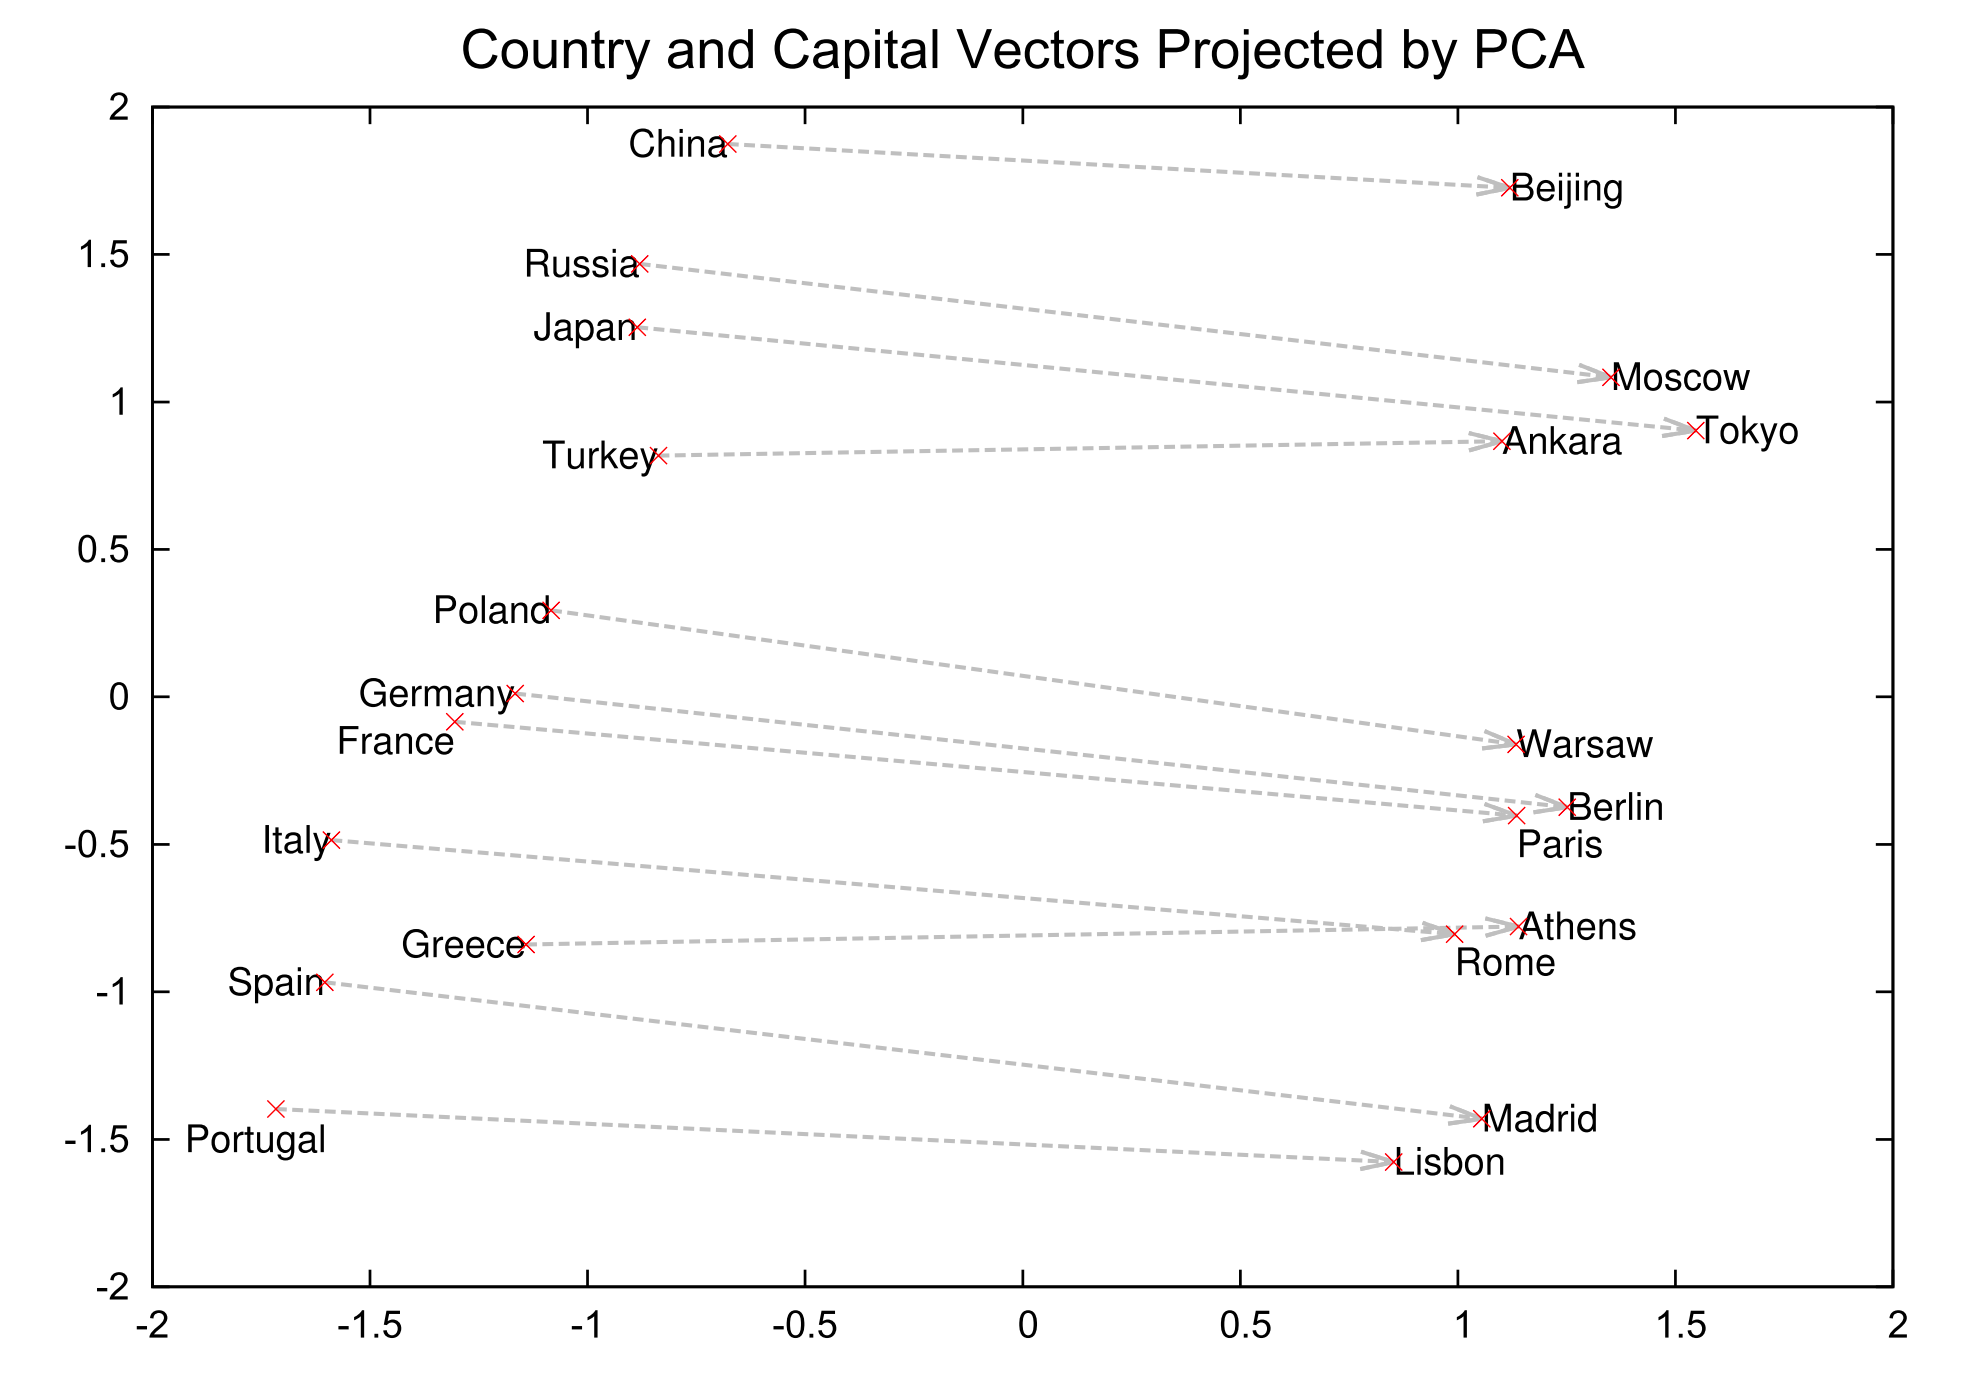
\includegraphics[width=\textwidth]{figures/word2vec-country-capital.png}
	\caption{Divdimensionāla PCA projekcija uzrāda attiecības starp valstu un galvaspilsētu jēdzientelpām \cite{colyer2016}}
	\label{fig:country-capital}%
\end{figure}

%distributed reprezentations
%http://www.cs.toronto.edu/~rgrosse/courses/csc321_2018/readings/L07%20Distributed%20Representations.pdf


\section{Daudzvalodīga jēdzientelpa}

Daudzvalodīgas jēdzientelpas no vienvalodīgām jēdzientelpām atšķiras ar to, ka uztver attiecības starp vārdiem no dažādām valodām.

Tā kā vienvalodīgas jēdzientelpas tiek trenētas tikai uz vienas valodas, tās nespēj notvert attiecības starp vārdiem dažādās valodās, un spēj raksturot tikai attiecības starp vārdiem vienā valodā, piemēram, vārds “suns" tiek reprezentēts kā vektors, kas jēdzientelpā ir tuvs citiem ar suņiem saistītiem vārdiem kā “kucēns" un “riet", bet nav sasaistīts ar suņiem saistītiem vektoriem citās valodās.

Turpretī daudzvalodīgas jēdzientelpas tiek trenētas uz paralēliem datiem - vienādas nozīmes tekstiem dažādās valodās. Tas ļauj notvert starpvalodu (\textit{cross-lingual}) sakarības starp līdzīgas nozīmes vārdiem kopējā jēdzientelpā, piemēram, vārdi “suns" un “dog" ("suns" angļu valodā) tiek reprezentēti kā tuvi vektori kopējā jēdzientelpā, kas norāda uz līdzīgu nozīmi. Daudzvalodīgas jēdzientelpas īpaši noder valodām ar mazākām treniņdatu kopām, jo palīdz tulkot un atgriezt informāciju starp valodām (\textit{cross-language information retrieval}) -- piemēram, atgriezt kādām vaicājumam angļu Vikipēdijas lapu, ja tai nav latviešu Vikipēdijas ekvivalenta. Pat tādām populārām valodām kā spāņu un hindi Vikipēdijas rakstu skaits ir būtiski mazāks par rakstu skaitu angļu valodas versijā (attiecīgi 26\% un 2.3\%), kā arī vairākums no šiem rakstiem ir īsāki, nekā to angliskās versijas. Turklāt gandrīz pusei no ne-angļu rakstiem nav attiecīgā analoga angļu versijā, visdrīzāk tāpēc, ka tie raksti ir veltīti specifiskai kulturālai vai ģeogrāfiskajai informācijai. Tas parāda nepieciešamību ņemt vērā saturu vairākās valodās, lai korekti un līdzvērtīgi pārstāvētu mazās valodas mašīnapmācības procesā \cite{roy2020}.


\section{Jēdzientelpu korpusi}


Lielo teksta korpusu un mašīnmācīšanās modeļu precizitātes vēsture ir cieši saistīta. Agrīnie mašīnmācīšanās algoritmi balstījās uz nelielām manuāli veidotām datu kopām, kas ierobežoja to efektivitāti. Viens no pirmajiem korpusiem bija \textit{Standard Sample of Present-Day American English}, plašāk pazīstams kā \textit{The Brown Corpus}, kas tika izdots 1964-1965. gadā un sastāvēja no apmēram viena miljona vārdu angļu teksta no dažādiem avotiem \cite{brown-corpus}, tas ir mazs apjoms teksta salīdzinot ar mūsdienās pieejamo.

Procesoru jaudas palielināšanās kopā ar datoru un interneta savienojuma pieejamību plašākai sabiedrībai ir radījuši labvēlīgu vidi izveidot un uzglabāt lielu daudzumu digitālo datu, tostarp teksta formā. Lieliem teksta korpusiem ir bijusi izšķiroša loma efektīvu mašīnmācīšanās modeļu izstrādē. Mašīnmācīšanās modeļu efektivitāte ir proporcionāla tiem pieejamo apmācības datu lielumam un kvalitātei. %source

Pirms lielu teksta korpusu pieejamības mašīnmācīšanās modeļi aprobežojās ar mazām un salīdzinoši vienkāršām datu kopām, tādēļ bija grūti sasniegt augstu precizitāti dabiskās valodas apstrādes uzdevumos. Mūsdienās lielos teksta korpusos kā Common Crawl un Wikipedia ir miljardiem vārdu vairākās valodās, kas ļauj modeļiem iemācīties ģenerēt cilvēkiem līdzīgu valodu.

Taču vai visas valodas ir līdzvērtīgi pārstāvētas korpusos? Viegli iztēloties, ka tādi lielie korpusi kā Common Crawl (kopš 2008. gada ievākti petabaiti datu no interneta mājaslapām, tostarp Vikipēdijas un Reddit) līdzvērtīgi pārstāv visu Zemes iedzīvotāju valodas. Taču valodu reprezentācija korpusos ir saistīta ar rakstītā teksta datu pieejamību šajā valodā, un neprecīzi atspoguļo cilvēku skaitu, kuri runā šajā valodā. Piemēram, valodai, kurā runā liels skaits cilvēku, korpusā var būt maz marķieru, ja šajā valodā ir maz digitāli pieejama rakstīta teksta \cite{bender2021}.

Tomēr dažādi faktori traucē visiem rakstīt tekstus internetā, kas vēlāk nokļūst korpusos, piemēram, rakstītneprasme, nabadzība, ierīču un interneta nepieejamība, karš utml. Tā rezultātā korpusos ir disproporcionāli pārstāvēti gados jaunāku lietotāju no attīstītajām valstīm drukāti teksti, piemēram, GPT-2 apmācības dati tika ievākti no Reddit, un pēc Pew Internet Research pētījuma 67\% Reddit lietotāju Amerikas Savienotajās Valstīs ir vīrieši un 64\% vecumā no 18 līdz 29 gadiem \cite{bender2021}.

Līdzīgi 87\% Vikipēdijas ierakstu veicēji ir vīrieši. Gandrīz puse dzīvo Eiropā un viena piektā daļa Ziemeļamerikā, salīdzinot ar 9.7\% un 4.8\% pasaules iedzīvotāju \cite{wikimedia2020}. Analizējot labojumus Vikipēdijas rakstos no 2001. līdz 2010. gadam, 1\% visbiežākie ierakstu veicēji uzrakstīja 77\% satura \cite{1percent}.

Korpusos tam ir vairākas praktiskas implikācijas gan sintaksē, gan semantikā. Piemēram, Vikipēdijas autors Brians Hendersons (\textit{Bryan Henderson}) 15 gados veica 90 tūkstošus labojumu, kur lielākā daļa izmaiņu ir no “comprised of" uz “comprised", kaut gan abas formas tiek pieņemtas un citos rakstiskos avotos “comprised of" ir izplatītāks (\ref{fig:distributed-representation} attēls). Tāpat BERT biežāk asociē cilvēkus ar invaliditāti ar negatīva sentimenta vārdiem un vairāki darbi to sasaista ar treniņu datu kopu īpašībām \cite{bender2021}. Pētīt negatīvu sentimentu valodu korpusos ir svarīgi, jo kompānijas reputācija ciestu, virtuālajam asistentam sniedzot atbildes ar negatīviem steriotipiem klientu apkalpošanas jomā.


\begin{figure}[h]
    \centering
    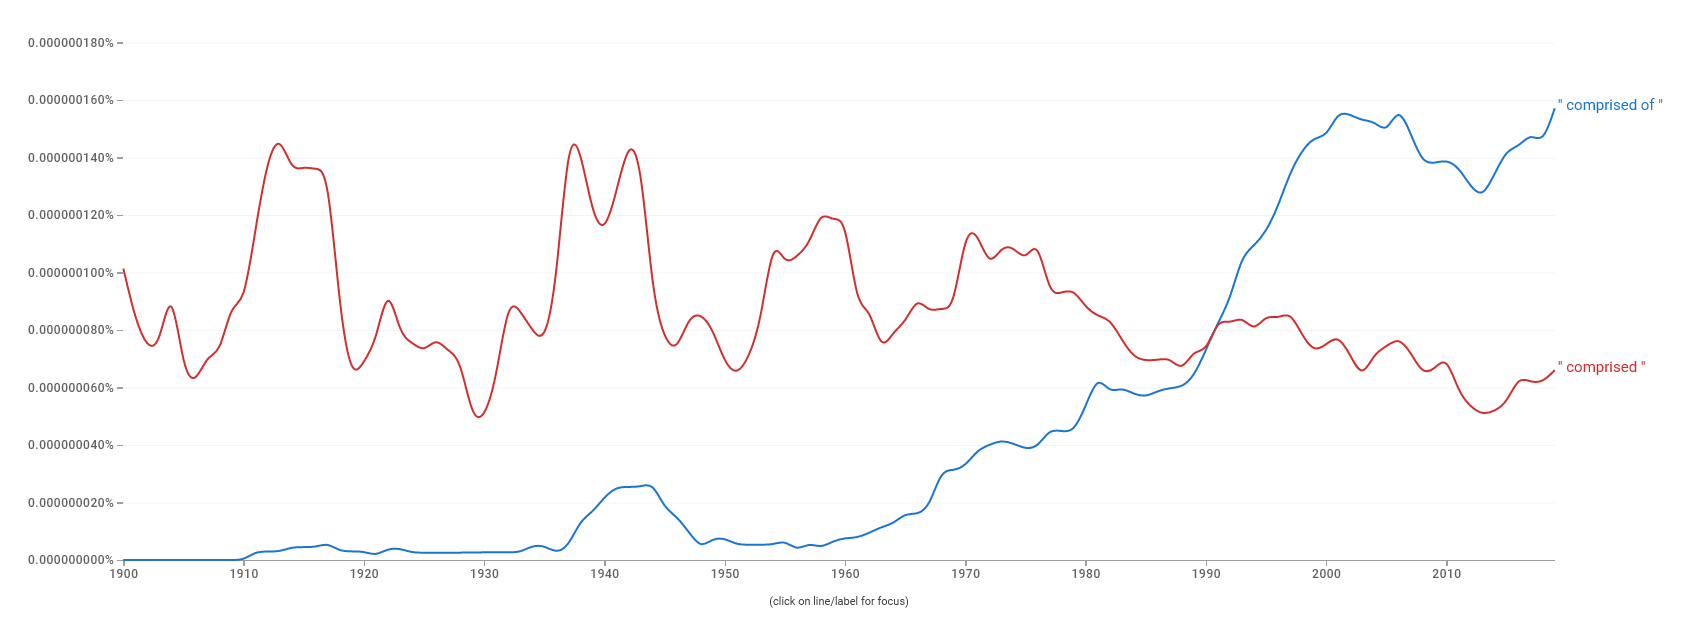
\includegraphics[width=\textwidth]{figures/comprised.png}
    \caption{Uz x ass attēloti gadi, uz y ass -- cik procentu no visiem vārdiem, kas ietverti angļu valodā rakstīto grāmatu korpusā (English 2019), ir “comprised of" (zilā līnija) un “comprised" (sarkanā līnija)? \cite{ngram-viewer}}
    \label{fig:comprised}
\end{figure}

Ar to tiek pierādīts, ka tekstu nav radījuši nejauši izvēlēta izlase cilvēku, tāpēc teksts nav neitrāls. Tiek paredzēts, ka virtuālos asistentus izmantos plašāks cilvēku loks nekā šobrīd internetā publicēto tekstu autori, tāpēc ir svarīgi, lai treniņdatos ir atbilstoši pārstāvēta potenciālo lietotāju valoda.


Latviešu marķieru daļa Common Crawl 100 korpusā ir atkarīga no daudziem faktoriem, tostarp latviešu satura daudzuma tīmeklī un korpusa konstruēšanā izmantotās izlases metodikas. Iespējams, ka latviešu teksta saturs korpusā ir pārāk vai nepietiekami pārstāvēts, salīdzinot ar tā izplatību tīmeklī vai proporcionāli latviešu valodā runājošo īpatsvaram.


Kas padara valodu par maz-resursu? Mazāks skaits vārdu un teikumu datu kopās, tātad mazāks skaits tokenu uz kuriem trenēt daudzvalodu jēdzientelpu modeli. Piemēram, Common Crawl-100 korpusā, uz kura trenēts XLM-R modelis, svahili un urdu valodās ir 275M un 730M tokenu attiecīgi, darbā izmantotajās - lietuviešu, latviešu, igauņu - ir 1835M, 1198M un 843M tokenu attiecīgi (\ref{tab:cc-100} tabula), tātad šīs datukopas kontekstā tās var uzskatīt par maz-resursu.


% Table generated by Excel2LaTeX from sheet 'cc-100'
\begin{table}[htbp]
    \centering
    \caption{Common Crawl-100 valodas un statistika: valodu saraksts ar marķieru (\textit{tokens}) skaitu (miljonos) un datu izmēru gibibaitos (GiB) katrai valodai}
    \begin{tabular}{llrr}
        \toprule
        ISO kods & Valoda     & Marķieri (M) & Izmērs (GiB) \\\midrule
        en       & angļu      & 55608        & 300.8        \\
        ru       & krievu     & 23408        & 278.0        \\
        lt       & lietuviešu & 1835         & 13.7         \\
        lv       & latviešu   & 1198         & 8.8          \\
        et       & igauņu     & 843          & 6.1          \\
        ur       & urdu       & 730          & 5.7          \\
        sw       & svahili    & 275          & 1.6          \\\bottomrule
    \end{tabular}
    \label{tab:cc-100}
\end{table}

\begin{figure}[h]
    \centering
    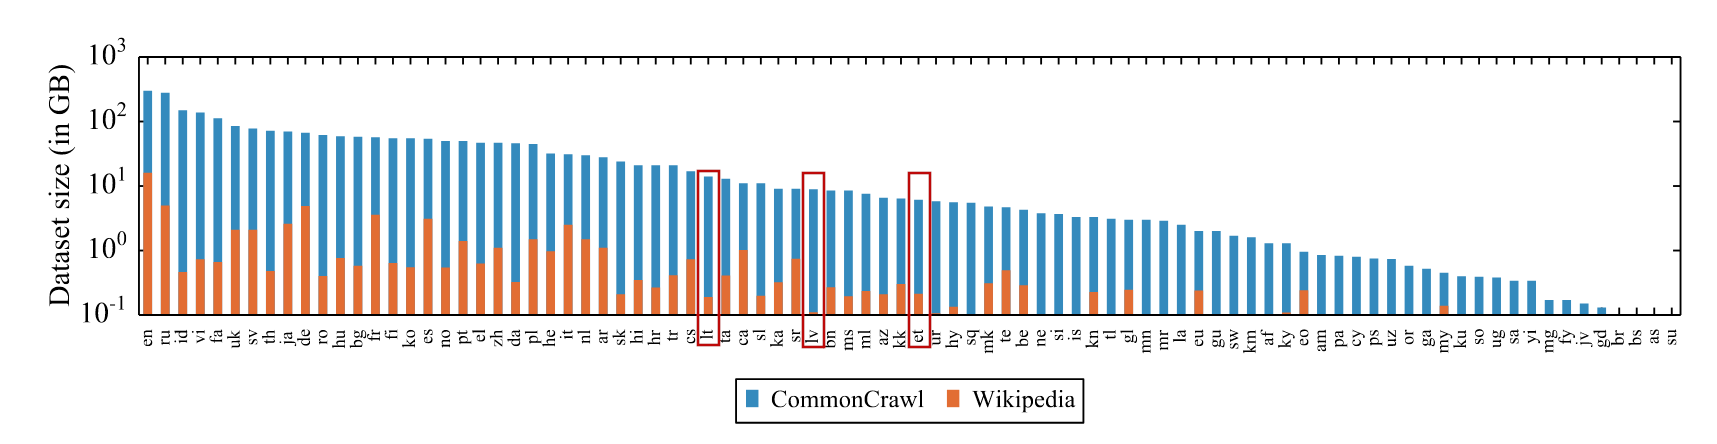
\includegraphics[width=\textwidth]{figures/dataset-size.png}
    \caption{Datu apjoms GiB (logaritmiskā skalā) valodām Wiki-100 korpusā, ko izmanto mBERT un XLM-100, un Common Crawl-100, ko izmanto XLM-R. Common Crawl-100 palielina datu apjomu par vairākām kārtām, jo īpaši maz-resursu valodās \cite{conneau2020} Grafikā ir iekļautas piecas konkrētas šajā darbā izmantotās valodas (atzīmētas ar sarkaniem taisnstūriem) parādīšanās secībā: angļu, krievu, lietuviešu, latviešu, igauņu.}
    \label{fig:dataset-size}
\end{figure}

